\documentclass{article}

% Language setting
% Replace `english' with e.g. `spanish' to change the document language
\usepackage[english]{babel}

% Set page size and margins
% Replace `letterpaper' with`a4paper' for UK/EU standard size
\usepackage[letterpaper,top=2cm,bottom=2cm,left=3cm,right=3cm,marginparwidth=1.75cm]{geometry}

% Useful packages
\usepackage{amsmath}
\usepackage{graphicx}
\usepackage{float}
\usepackage[colorlinks=true, allcolors=blue]{hyperref}

\title{Design Document for memFS (CL Project)}
\author{
      Gana Jayant Sigadam \\
      Roll No: 24CS60R12 \\
}

\begin{document}
\maketitle


\section{Overview}

\texttt{memFS} is a Command Line Interface (CLI) tool designed to create files in-memory and perform high-speed operations on them. Once the program terminates, all the files created in memory are lost. This makes \texttt{memFS} particularly useful for testing scenarios where temporary file operations are required without impacting the actual disk.

\subsection*{Key Features}
\begin{itemize}
    \item Fast in-memory file operations: Files are created, written, and deleted directly in memory, enabling faster operations compared to disk I/O.
    \item Temporary storage: All in-memory files are lost once the program ends, ensuring no residual files on disk.
    \item Concurrency: Supports multi-threaded operations to handle multiple files simultaneously, enhancing performance for bulk operations.
\end{itemize}

\subsection*{Implementation Details}
\begin{itemize}
    \item Language and Concepts: The tool is implemented in \textbf{C++} and leverages \textbf{multi-threading} to achieve high performance.
    \item Command Parsing: To handle user input, a custom parser has been implemented. This parser validates commands and arguments, ensuring correct execution. The code for the parser can be found in the \texttt{CommandInterpreter.hpp} file.
    \item Concurrency for Operations:
    \begin{itemize}
        \item Multi-threading is used to optimize \textbf{create}, \textbf{write}, and \textbf{delete} operations.
        \item Users can specify multiple files for operations, and threads handle these operations in parallel, ensuring efficiency.
    \end{itemize}
\end{itemize}

\subsection*{Flow Diagram}
To better understand the process flow of the \texttt{memFS} tool, refer to the flow diagram below.

\begin{figure}[H]
    \centering
    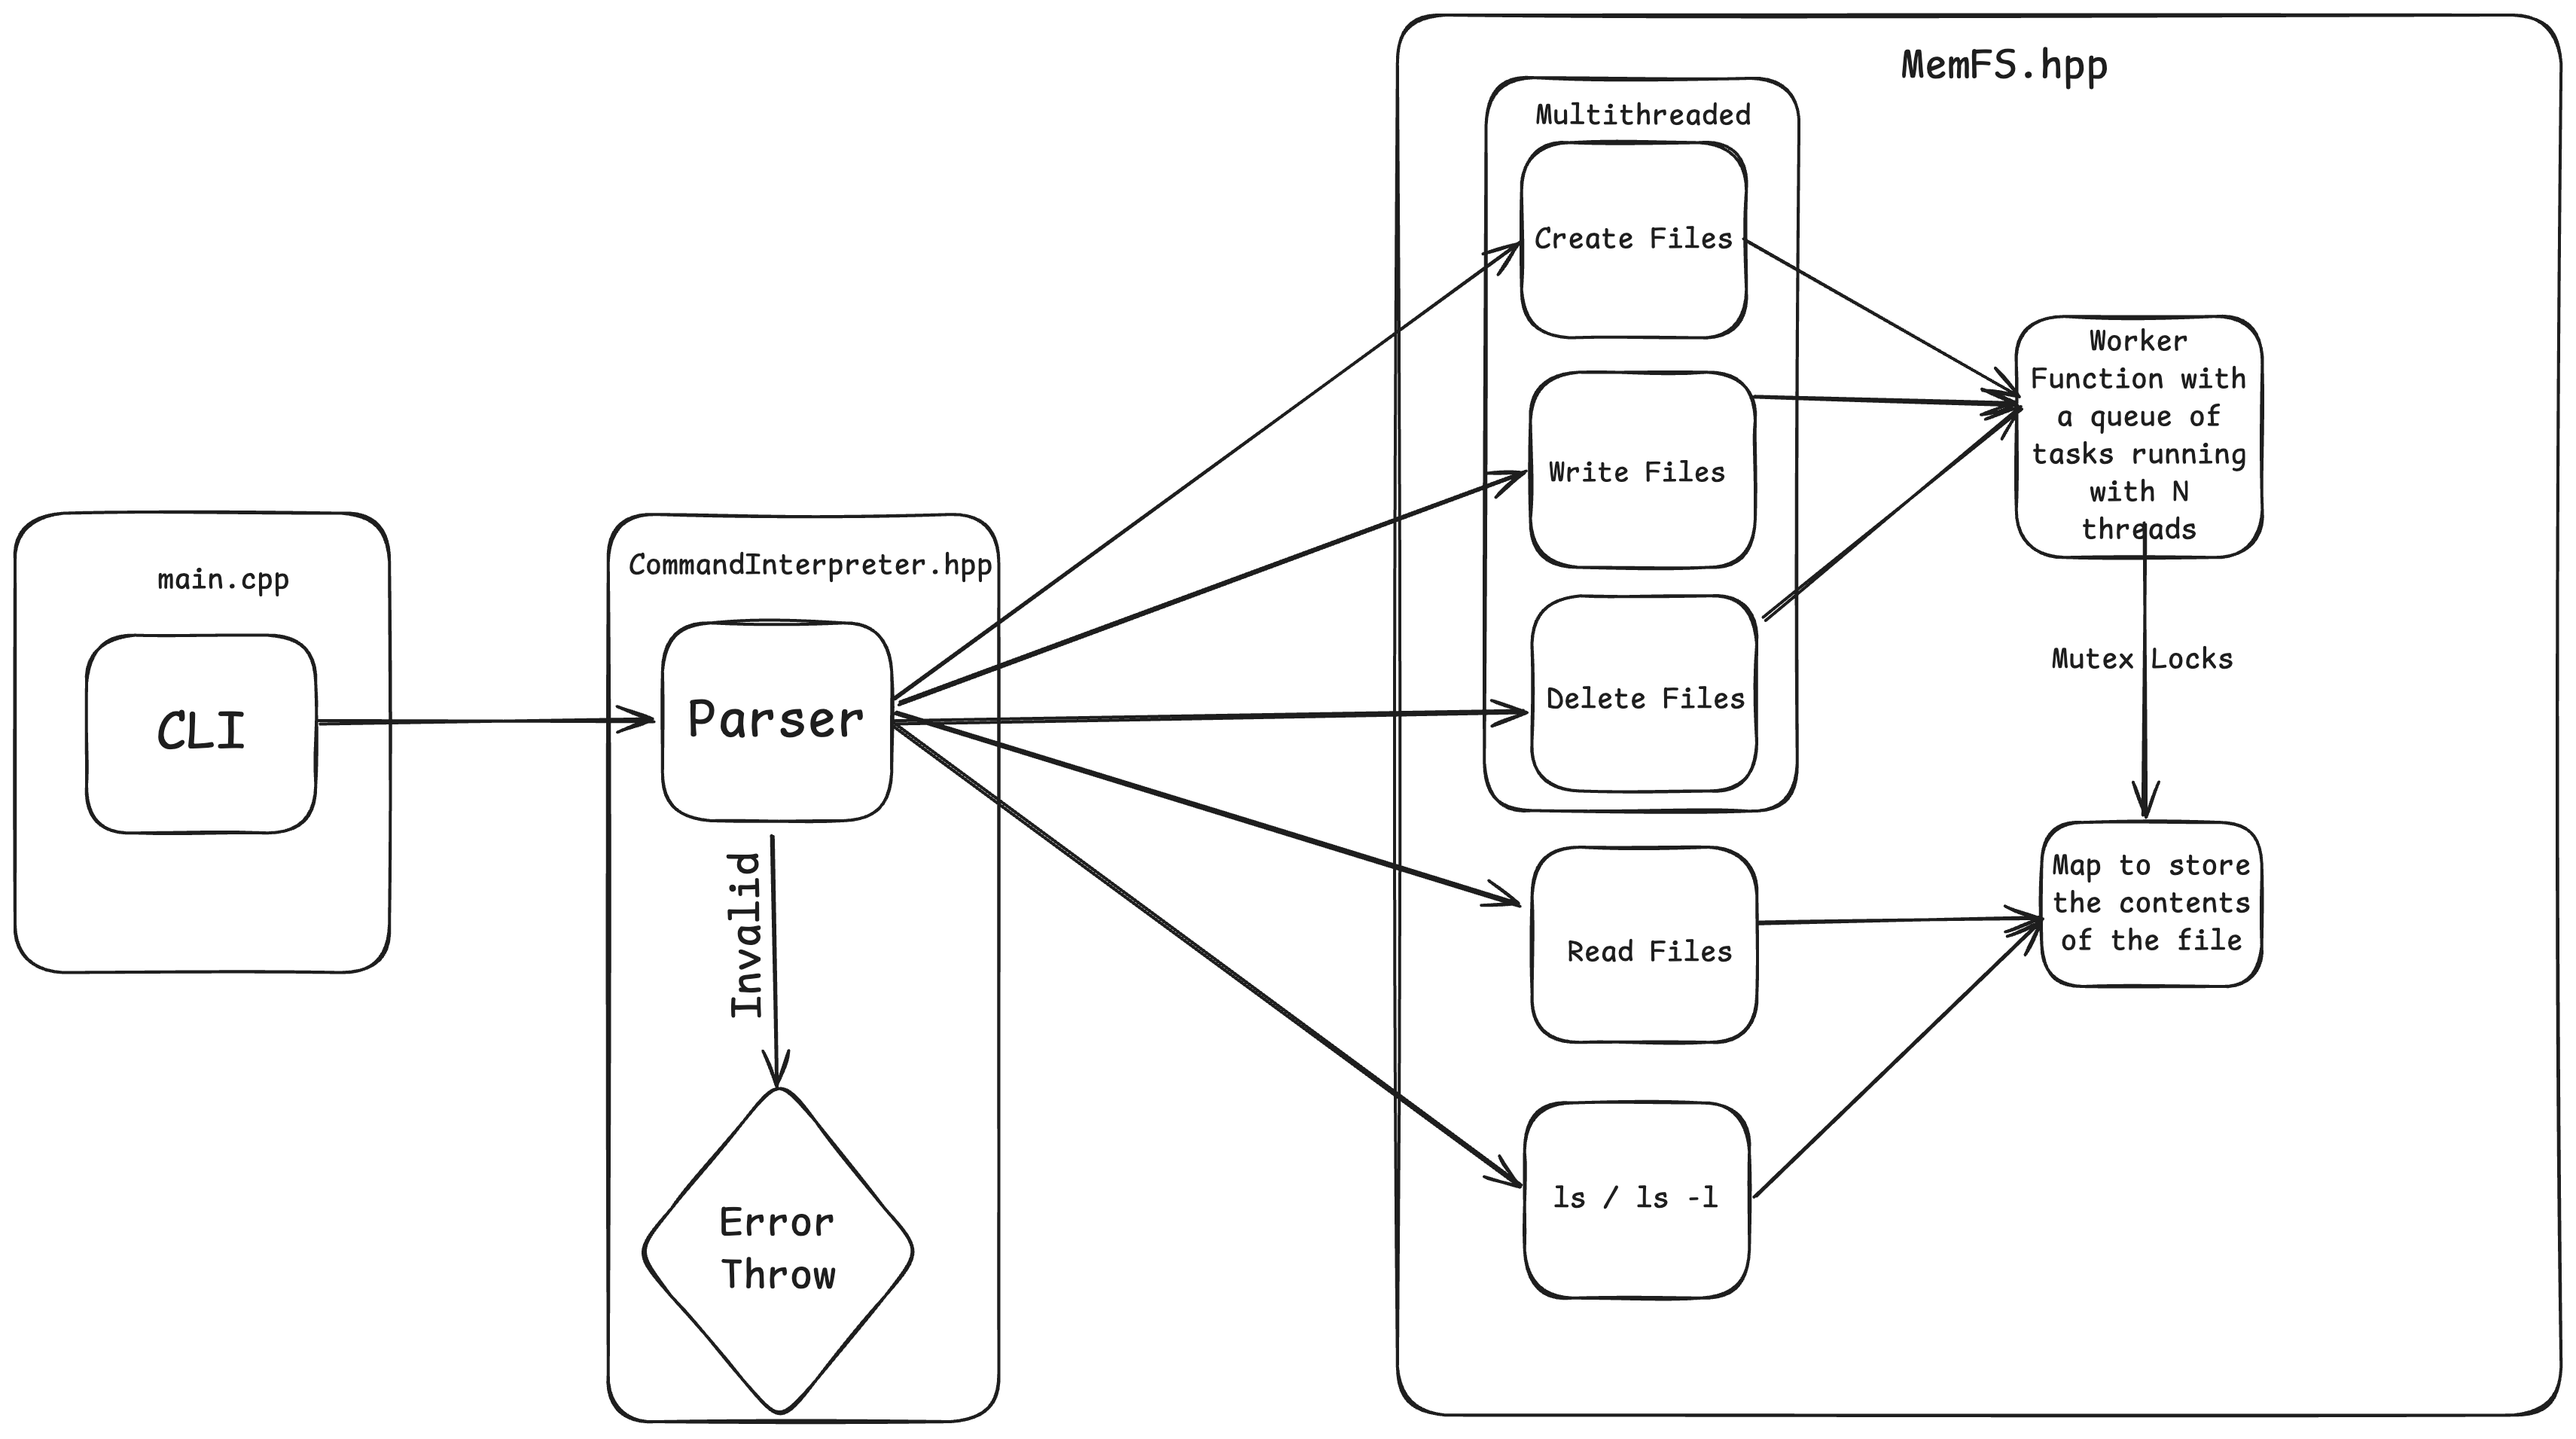
\includegraphics[width=0.8\textwidth]{./pictures/flow_diagram.png}
    \caption{\label{fig:flow_diagram}Flow Diagram of \texttt{memFS}}
\end{figure}


\section{Context}
Why we need this tool?
\begin{itemize}
    \item Since RAM is significantly faster than traditional storage, operations such as reading, writing, creating, or deleting files are much quicker in MemFS.
    \item Traditional filesystems incur latency due to physical storage access, disk scheduling, and caching. MemFS bypasses these layers, reducing overhead.
    \item MemFS is useful for testing purposes where we need to create files and perform operations on them without actually creating them on disk.
\end{itemize}

\section{Goals \& Non-Goals}

\subsection{Goals}
\begin{itemize}
      \item Create files in-memory.
      \item Write data to files in-memory.
      \item Read data from files in-memory.
      \item Delete files in-memory.
      \item Faster operations on files.
\end{itemize}

\subsection{Non-Goals}
\begin{itemize}
      \item This tool is not intended to store files permanently.
      \item This tool is not intended to store large files.
\end{itemize}

\section{Proposed Solution}

\subsection{Parsing Commands}
First, I have implemented a command parser that validates user input and extracts the command and arguments. The parser ensures that the command is valid and the arguments are correctly formatted using regex and matching techniques. The parser is implemented in the \texttt{CommandInterpreter.hpp} file.


\subsection{MemFS Logic}

\subsubsection{Data Structuring for Files}
To store files in memory, I have used a \texttt{std::map} data structure where the key is the file name and the value is the \texttt{File} object. The \texttt{File} object contains the content, size, create time, and last modified time of the file which will be used for operations.

\noindent This acts as a critical section for the threads to access the file system. The critical section is protected by a mutex to ensure thread safety.

\noindent Worker threads are spawned to handle file operations concurrently. The number of worker threads can be passed in the constructor of the \texttt{MemFS} class.

\noindent This worker threads constantly check are there any operations in the queue. If there are any operations, they will pick the operation and execute it.

\subsubsection{Worker Queue}
The worker queue is a \texttt{std::queue} data structure that stores the operations to be performed on files. The worker threads continuously check the queue for operations. If an operation is present, the worker thread picks the operation and processes it and after processing it let's the main thread know that the operation is completed using \texttt{std::condition\_variable}.

\subsubsection{Create Operation}
\noindent This operation takes multiple file names as input and creates files in memory. The files are stored in the \texttt{std::map} data structure. Each file is added to the worker queue for processing. Corresponding errors are displayed if the file already exists.

\subsubsection{Write Operation}
\noindent This operation takes multiple file names and data as input and writes the data to the files in memory. The files are updated in the \texttt{std::map} data structure. Each file is added to the worker queue for processing. Corresponding errors are displayed if the file does not exist.

\subsubsection{Read Operation}
\noindent This operation is single-threaded and takes one filename as input. It reads the content of the file from memory and displays it. Corresponding errors are displayed if the file does not exist.

\subsection{Delete Operation}
\noindent This operation takes multiple file names as input and deletes the files from memory. The files are removed from the \texttt{std::map} data structure. Each file is added to the worker queue for processing. Corresponding errors are displayed if the file does not exist.

\subsection{Ls Operation}
\noindent This operation is single-threaded and displays the list of files present in memory. There is special flag \texttt{-l} which will display the detailed information of the files.

\section{Benchmarking}
For the benchmarking of the tool please refer to the Benchmarking document.

\section{Usage of the tool}
Please refer to the README file for the usage of the tool.

\section{Open Questions}
The futures scope of the project is to implement the following features:
\begin{itemize}
    \item Implement a lock-free data structure for file operations essentially a atomic hash map.
    \item Implementing actual file system with directory structure \& additional commands like  \texttt{cd}, \texttt{cp}.
\end{itemize}


\end{document}
